\taskpic{Стеклянная призма, имеющая в сечении равнобедренный
  треугольник, касается своим основанием поверхности воды. Луч света,
  идущий вдоль поверхности воды перпендикулярно оси призмы,
  преломляясь на первой поверхности призмы, испытывает полное
  внутреннее отражение от водной поверхности, преломляется на второй
  поверхности и вновь выходит в воздух. Показатели преломления стекла
  и воды равны $n_1$ и $n_2$ соответственно. Найдите минимальный угол
  $\theta$ --- угол в основании
  призмы. }{
  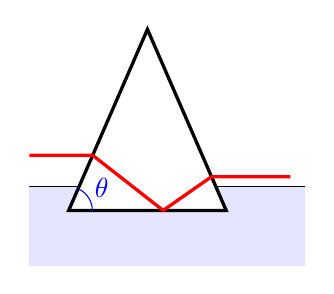
\begin{tikzpicture}
    \filldraw[blue!10] (0.5,1.5) rectangle (4,0.5);
    \draw (0.5,1.5) -- (4,1.5);
    \filldraw[fill=white,draw=black,very thick] (1,1.2) -- (3,1.2) --
    (2,3.5) -- cycle;
    \draw[very thick,red] (0.5,1.9) -- (intersection of 1,1.2--2,3.5 and
    0,1.9--4,1.9) -- (2.2,1.2) -- (intersection of 2.2,1.2--27:2cm and
    2,3.5--3,1.2) -- ++(0:1cm);
    \draw[blue] (1.3,1.2) arc (0:atan(2.3):0.3cm);
    \draw[blue] (1.42,1.48) node {$\theta$};
  \end{tikzpicture}
}